\chapter{Cài đặt hệ điều hành cho Raspberry Pi}
\section{Chuẩn bị}
\subsection{Phần cứng}
\begin{list}{--}{}
\item Máy tính Raspberry Pi: bạn có thể sử dụng Model $A$, $B$, $A+$, $B+$, $Pi~2$, $Pi~3$, $Pi Zero$.
\begin{figure}[!h]
\begin{center}
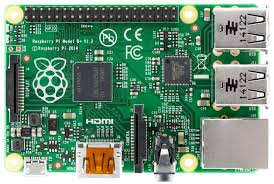
\includegraphics[scale=.5]{setup-os/images/Pi-H}
\end{center}
\caption{Raspberry Pi model B+}
\end{figure}
\item Thẻ nhớ SD: Dung lượng 4GB trở lên, tốc độ cao. Nên sử dụng thẻ nhớ có dung lượng $8GB$. Có thể sử dụng thêm Adapter (tùy theo phiên bản Pi mà bạn sử dụng).
\begin{figure}[!h]
\begin{center}
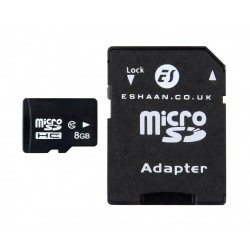
\includegraphics[scale=.4]{setup-os/images/SD-H}
\end{center}
\caption{Thẻ nhớ SD và Adapter}
\end{figure}
\item Nguồn điện cấp cho Pi hoạt động: nguồn DC $5V-1A$
\item Các ngoại vi khác: dây kết nối HDMI (hoặc cáp VGA và cáp chuyển đổi HDMI to VGA), màn hình có cổng HDMI (hoặc hoặc màn hình có cổng VGA), chuột, bàn phím, dây kết nối mạng.
\item[$\ast$] Nếu không có các thiết bị ngoại vi trên thì sử dụng các loại cáp truyền nhận dữ liệu giữa Pi và máy tính cũng có thể thực hiện được, ví dụ: RS232, PL2303.
\end{list}
\subsection{Phần mềm}
\begin{list}{--}{}
\item Phần mềm Format thẻ nhớ, ví dụ: SDFormatter.

Địa chỉ: \verb|https://www.sdcard.org/downloads/formatter_4/|
\item Phần mềm ghi hệ điều hành vào thẻ nhớ, ví dụ: Win32DiskImage.

Địa chỉ: \verb|https://sourceforge.net/projects/win32diskimager/|
\item Hệ điều hành: Chọn một trong hai hệ điều hành sau để tải về máy.
\begin{list}{+}{}
\item Trong phần này mình sử dụng hệ điều hành Raspbian.

Địa chỉ: \verb|https://www.raspberrypi.org/downloads/raspbian/|

\item Cài đặt bằng NOOBS: tích hợp nhiều hệ điều hành vào một gói, bạn thích sử dụng hệ điều hành nào thì chọn hệ điều hành đó.

Địa chỉ: \verb|https://www.raspberrypi.org/downloads/noobs/|
\end{list}
\end{list}
\section{Cài đặt hệ điều hành}
Bạn chọn một trong các cách sau để cài đặt.
\subsection{Cài đặt hệ điều hành Raspbian}
\begin{list}{--}{}
\item Cài đặt các phần mềm ở phần chuẩn bị, ví dụ: \verb|SDFormatter| và \verb|Win32DiskImage|.
\item Giải nén thư mục chứ hệ điều hành Raspbian (file .zip) được file \verb|.img|.
\item Mở phần mềm \verb|SDFormatter|, định dạng lại thẻ nhớ chuẩn bị ghi hệ điều hành lên. Chọn \verb|Format|. Thông báo xuất hiện chọn YES.
\begin{figure}[!h]
\begin{center}
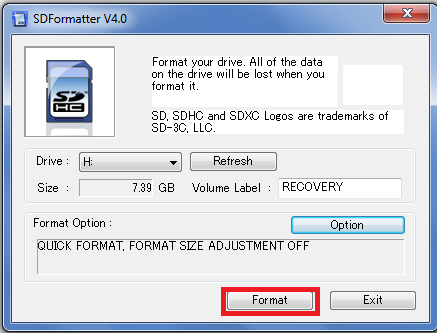
\includegraphics[scale=.4]{setup-os/images/SDFormatter}
\end{center}
\caption{Format lại thẻ nhớ để cài đặt hệ điều hành}
\end{figure}
\item Mở phần mềm \verb|Win32DiskImage| để ghi hệ điều hành vào thẻ nhớ, chọn đường dẫn đến file \verb|.img| đã giải nén ở bước trên. Chọn \verb|Write|. Thông báo xuất hiện chọn YES.
\begin{figure}[!h]
\begin{center}
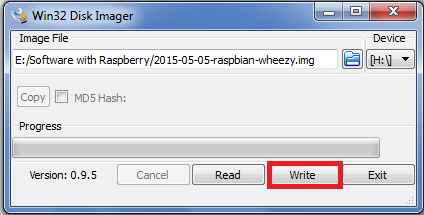
\includegraphics[scale=.5]{setup-os/images/Win32DiskImage}
\end{center}
\caption{Ghi hệ điều hành vào thẻ nhớ}
\end{figure}
\item Đợi cho quá trình ghi hệ điều hành hoàn thành là được.
\item Gắn thẻ nhớ vào Pi, kết nối màn hình, chuột, bàn phím, cấp nguồn khởi động và tiến hành một số cài đặt cần thiết khác.
\end{list}
\subsection{Cài đặt hệ điều hành Raspbian bằng NOOBS}
Khi cài đặt hệ điều hành bằng bản NOOBS, nó cũng có chứa hệ điều hành Raspbian, bạn có thể cài đặt hệ điều hành Raspbian bằng cách này.\\

Muốn có nhiều hệ điều hành khác được chọn thì bạn cần có kết nối Internet (sử dụng dây LAN).
\begin{list}{--}{}
\item Cài đặt các phần mềm ở phần chuẩn bị, ví dụ: \verb|SDFormatter| (không cần sử dụng phần mềm ghi hệ điều hành).
\item Giải nén thư mục chứa hệ điều hành trong bản NOOBS (file .zip).
\item Mở phần mềm \verb|SDFormatter|, định dạng lại thẻ nhớ chuẩn bị chép hệ điều hành lên. Chọn \verb|Format|. Thông báo xuất hiện chọn YES.
\begin{figure}[!h]
\begin{center}
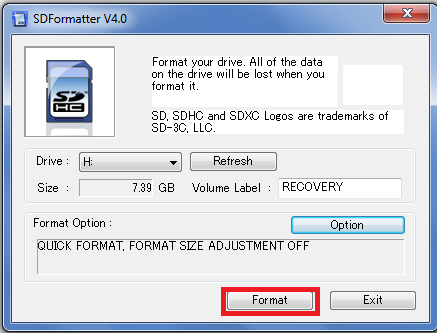
\includegraphics[scale=.4]{setup-os/images/SDFormatter}
\end{center}
\caption{Format lại thẻ nhớ để cài đặt hệ điều hành}
\end{figure}
\item Copy toàn bộ nội dung trong thư mục đã giải nén ở trên (của bản NOOBS) vào thẻ nhớ.
\item Gắn thẻ nhớ vào Pi, kết nối màn hình, chuột và bàn phím (hoặc các phương pháp tương đương khác), sẽ có một danh sách các hệ điều hành được được ra, bạn chọn hệ điều hành muốn cài đặt rồi nhấn \verb|Install| sau đó đợi quá trình cài đặt xong, khởi động lại Pi là hoàn thành.
\begin{figure}[!h]
\begin{center}
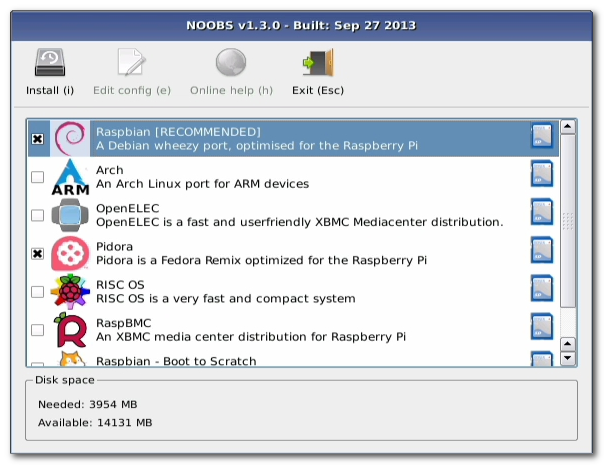
\includegraphics[scale=.5]{setup-os/images/NOOBS}
\end{center}
\caption{Các hệ điều hành trong bản NOOBS}
\end{figure}
\item Sau khi cài đặt hệ điều hành xong, tiến hành một số cài đặt cần thiết khác.
\end{list}
\section{Thiết lập ban đầu cho Raspberry Pi}
Sau khi cài đặt và khởi động, bạn có thể muốn thiết lập lại các cài đặt mặc định của hệ điều hành sao cho phù hợp với bạn. Sau khi thiết lập xong, reset lại Pi: \verb|sudo reboot|\\

Thực hiện lệnh: \verb|sudo raspi-config| để tiến hành cài đặt. Các tùy chọn thiết lập như hình dưới:
\begin{figure}[!h]
\begin{center}
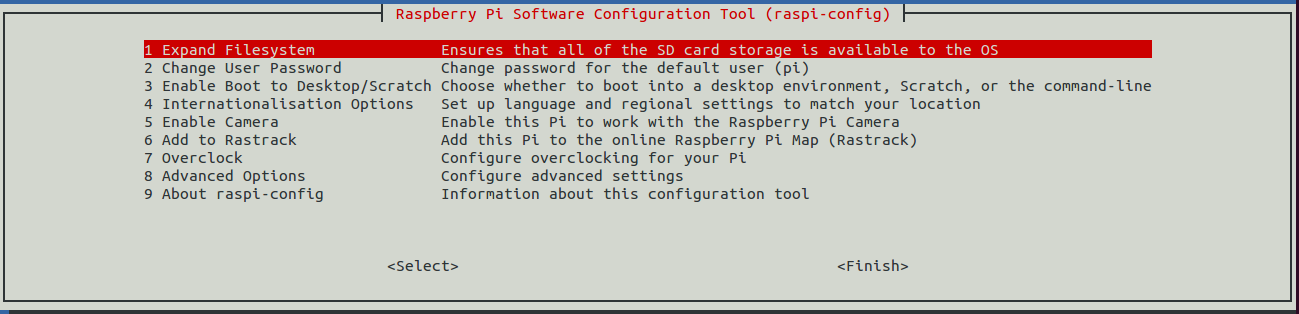
\includegraphics[scale=.35]{setup-os/images/raspi}
\end{center}
\caption{Các tùy chọn thiết lập cho Pi}
\end{figure}
\subsection{Thiết lập ngôn ngữ, múi giờ và kiểu bàn phím}
Thay đổi ngôn ngữ, múi giờ, kiểu bàn phím: \verb|Internationalisation Options|, được các lựa chọn sau:
\begin{figure}[!h]
\begin{center}
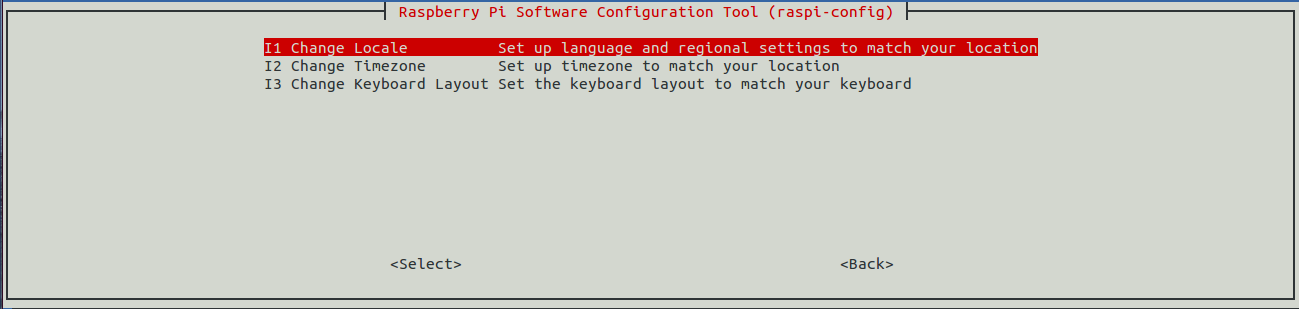
\includegraphics[scale=.35]{setup-os/images/Time}
\end{center}
\caption{Các tùy chọn thiết lập ngôn ngữ, múi giờ, kiểu bàn phím}
\end{figure}
\begin{list}{--}{}
\item Chọn \verb|Change Locale|: để thay đổi ngôn ngữ.

Đổi \verb|en_GB.UTF-8 UTF-8| thành \verb|en_US.UTF-8 UTF-8 | (sử dụng dấu cách \verb|space| để chọn hoặc bỏ chọn).
\begin{figure}[!h]
\begin{center}
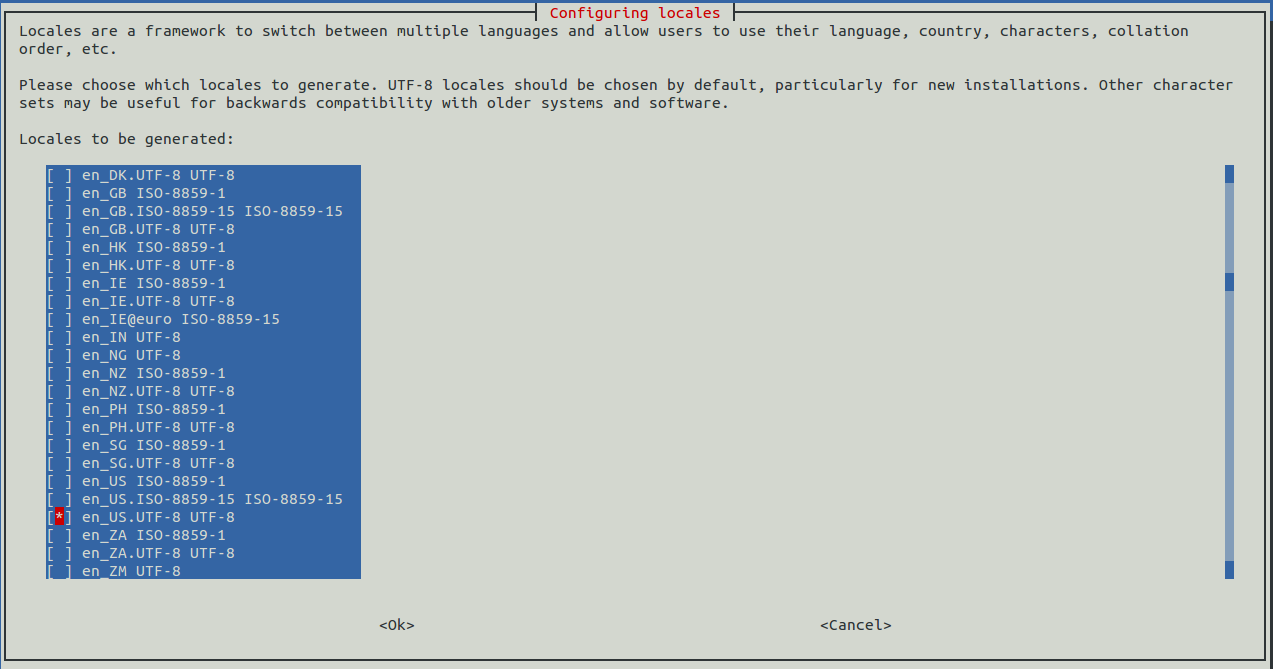
\includegraphics[scale=.35]{setup-os/images/lang}
\end{center}
\caption{Thay đổi ngôn ngữ thành \textsf{en\_US.UTF-8 UTF-8}}
\end{figure}
\item Chọn \verb|Change TimeZone|: để thay đổi múi giờ.

Chọn \verb|Asia| rồi chọn tiếp \verb|Ho_Chi_Minh|.
\begin{figure}[!h]
\begin{center}
\subfloat[Chọn \textsf{Asia}]
  {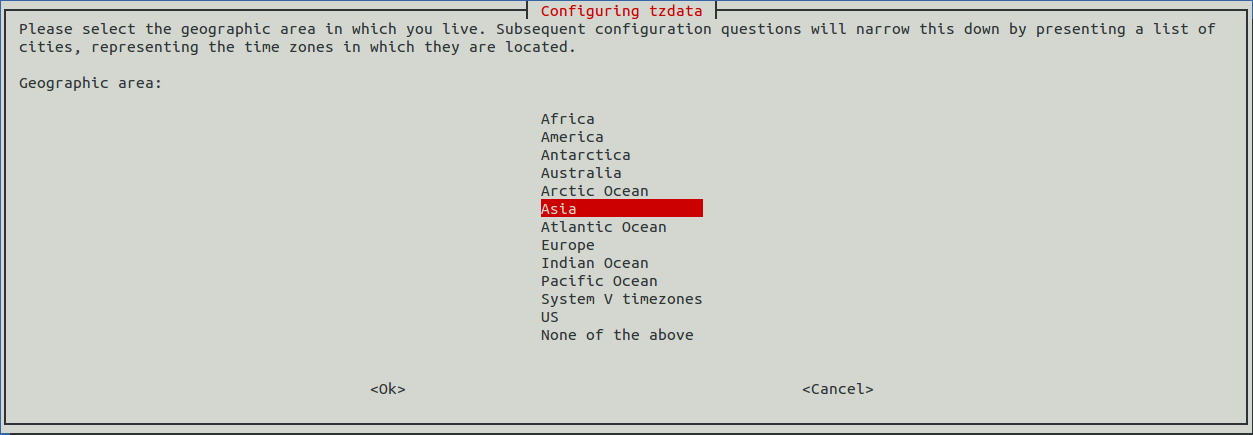
\includegraphics[scale=.35]{setup-os/images/time-zone}}\\
\subfloat[Chọn \textsf{Ho\_Chi\_Minh}]
  {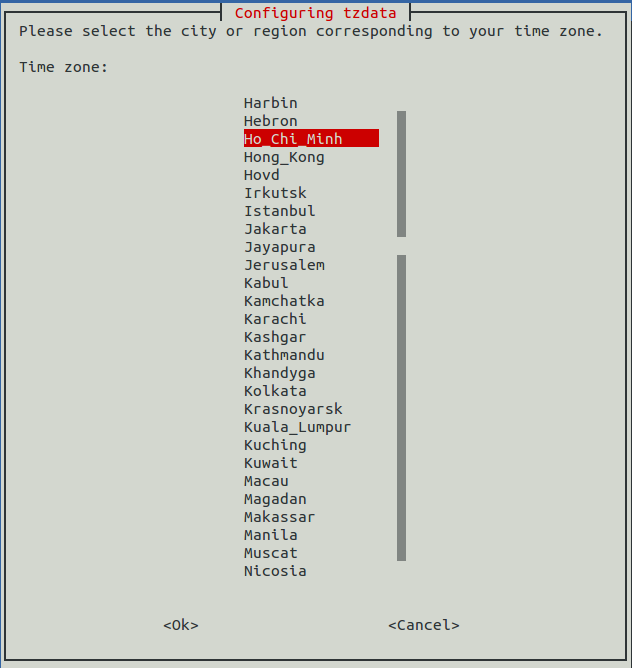
\includegraphics[scale=.35]{setup-os/images/time-zone-2}}
\end{center}
\caption{Thay đổi múi giờ}
\end{figure}
\newpage
\item Thay đổi kiểu bàn phím, dùng lệnh:
\begin{lstlisting}[language=bash]
$ sudo nano /etc/default/keyboard
\end{lstlisting}
Nội dung file như sau:
\begin{lstlisting}[language=bash]
# KEYBOARD CONFIGURATION FILE

# Consult the keyboard(5) manual page.

XKBMODEL="pc105"
XKBLAYOUT="gb"
XKBVARIANT=""
XKBOPTIONS=""

BACKSPACE="guess"
\end{lstlisting}

Đổi các khai báo sau: \verb|pc105| thành \verb|pc104| và \verb|gb| thành \verb|us|, sau khi thay đổi nội dung như sau:
\begin{lstlisting}[language=bash]
# KEYBOARD CONFIGURATION FILE

# Consult the keyboard(5) manual page.

XKBMODEL="pc104"
XKBLAYOUT="us"
XKBVARIANT=""
XKBOPTIONS=""

BACKSPACE="guess"
\end{lstlisting}

Nhấn \verb|Ctrl + X + Y| và \verb|Enter| để lưu nội dung thay đổi.
\item[$\ast$] Để thoát khỏi \verb|raspi-config| nhấn phím \verb|Esc|.
\end{list}
\subsection{Cập nhật Raspberry Pi}
\begin{list}{--}{}
\item Kiểm tra cập nhật:
\begin{lstlisting}[language=bash]
$ sudo apt-get update
\end{lstlisting}
\item Tiến hành cập nhật:
\begin{lstlisting}[language=bash]
$ sudo apt-get upgrate
\end{lstlisting}
Nếu có các thay đổi bạn cần chọn \verb|Y| để bắt đầu cặp nhật.
\item Cập nhật \verb|firmware|:
\begin{lstlisting}[language=bash]
$ sudo rpi-update
\end{lstlisting}
\end{list}
\subsection{Thiết lập dòng cung cấp cho ngõ ra USB}
Dòng mặc định là $600mA$, cần tăng dòng lên $1200mA$ để sử dụng các USB.
\begin{list}{--}{}
\item Mở file \verb|config.txt| để thay đổi nội dung:
\begin{lstlisting}[language=bash]
$ sudo nano /boot/config.txt
\end{lstlisting}
\item Thêm nội dung sau vào cuối file \verb|config.txt| (dùng \verb|Ctrl + V| để di chuyển nhanh):
\begin{lstlisting}[language=bash]
max_usb_current=1
\end{lstlisting}
Nhấn \verb|Ctrl + X + Y| để lưu thay đổi.
\end{list}
\subsection{Bật SSH}
\verb|SSH| cho phép điều khiển Pi từ xa thông qua mạng Internet.
\begin{list}{--}{}
\item Chọn \verb|Advanced Options|: hình \ref{Fig:Advanced Options}.
\begin{figure}[!h]
\begin{center}
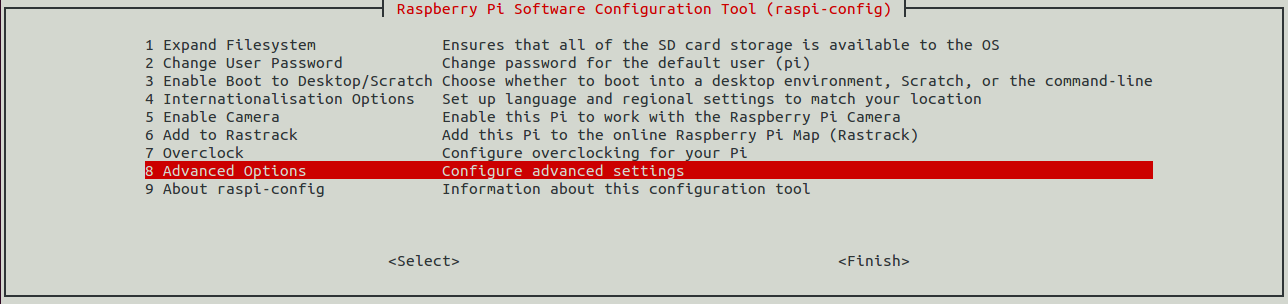
\includegraphics[scale=.35]{setup-os/images/ssh-setup}
\end{center}
\caption{Mở các tùy chọn nâng cao \textsf{Advanced Options}}\label{Fig:Advanced Options}
\end{figure}
\item Chọn \verb|A4 SSH|: hình \ref{Fig:A4 SSH}.
\begin{figure}[!h]
\begin{center}
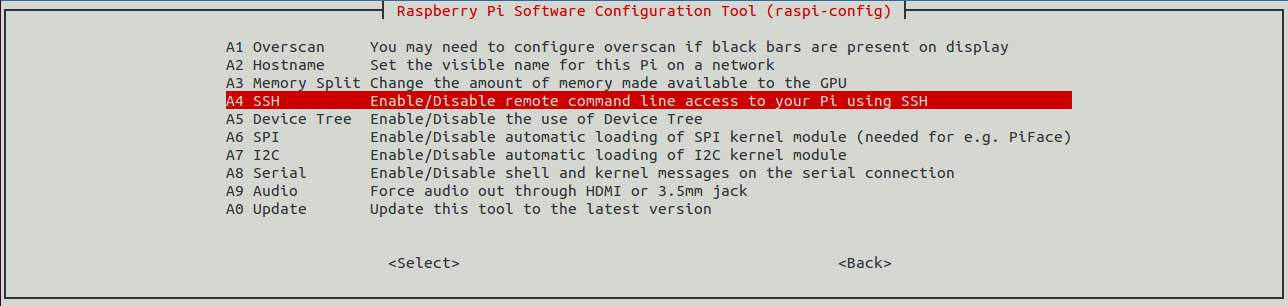
\includegraphics[scale=.35]{setup-os/images/a4-ssh}
\end{center}
\caption{Chọn  \textsf{A4 SSH}}\label{Fig:A4 SSH}
\end{figure}
\item Chọn \verb|Enable|: hình \ref{Fig:Enable}.
\begin{figure}[!h]
\begin{center}
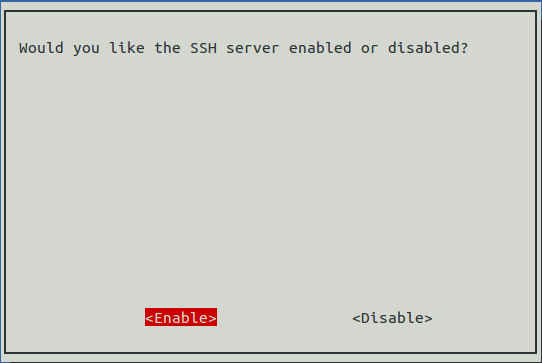
\includegraphics[scale=.35]{setup-os/images/a4-ssh-2}
\end{center}
\caption{Chọn \textsf{Enable}}\label{Fig:Enable}
\end{figure}
\end{list}